\section{Uzupełnianie danych}

W tworzonym systemie założono, że powinny istnieć pewne informacje, które dla klientów i wykonawców zawsze są określone. Przykładem tego jest imię i nazwisko. Użytkownik, który ich nie określił, nie powinien być dopuszczony do głównych funkcjonalności aplikacji. Dla wykonawców wśród takich obligatoryjnych elementów znajduję się również obszar działania oraz przynajmniej jedna świadczona usługa. Bez tego nie mogliby otrzymywać żadnych zleceń i byliby nieprzydatni.

W celu żądania uzupełnienia danych stworzone zostały ekrany, które przedstawiono na rysunku \ref{fig:setup}. Są one wyświetlane po rejestracji i uniemożliwiają użytkownikom przejście dalej tak długo, jak niezbędne informacje nie są kompletne. Gdy zostaną już podane, to nie ma możliwości ich usunięcia, a dostępna jest jedynie aktualizacja. Jeśli wykorzystywane jest logowanie za pomocą Google, to imię i nazwisko zostaje automatyczne przepisane z profilu na tej platformie i danych do uzupełnienia jest mniej.

\begin{figure}[ht]
  \centering
  \begin{subfigure}[t]{0.33\textwidth}
    \centering
    \fbox{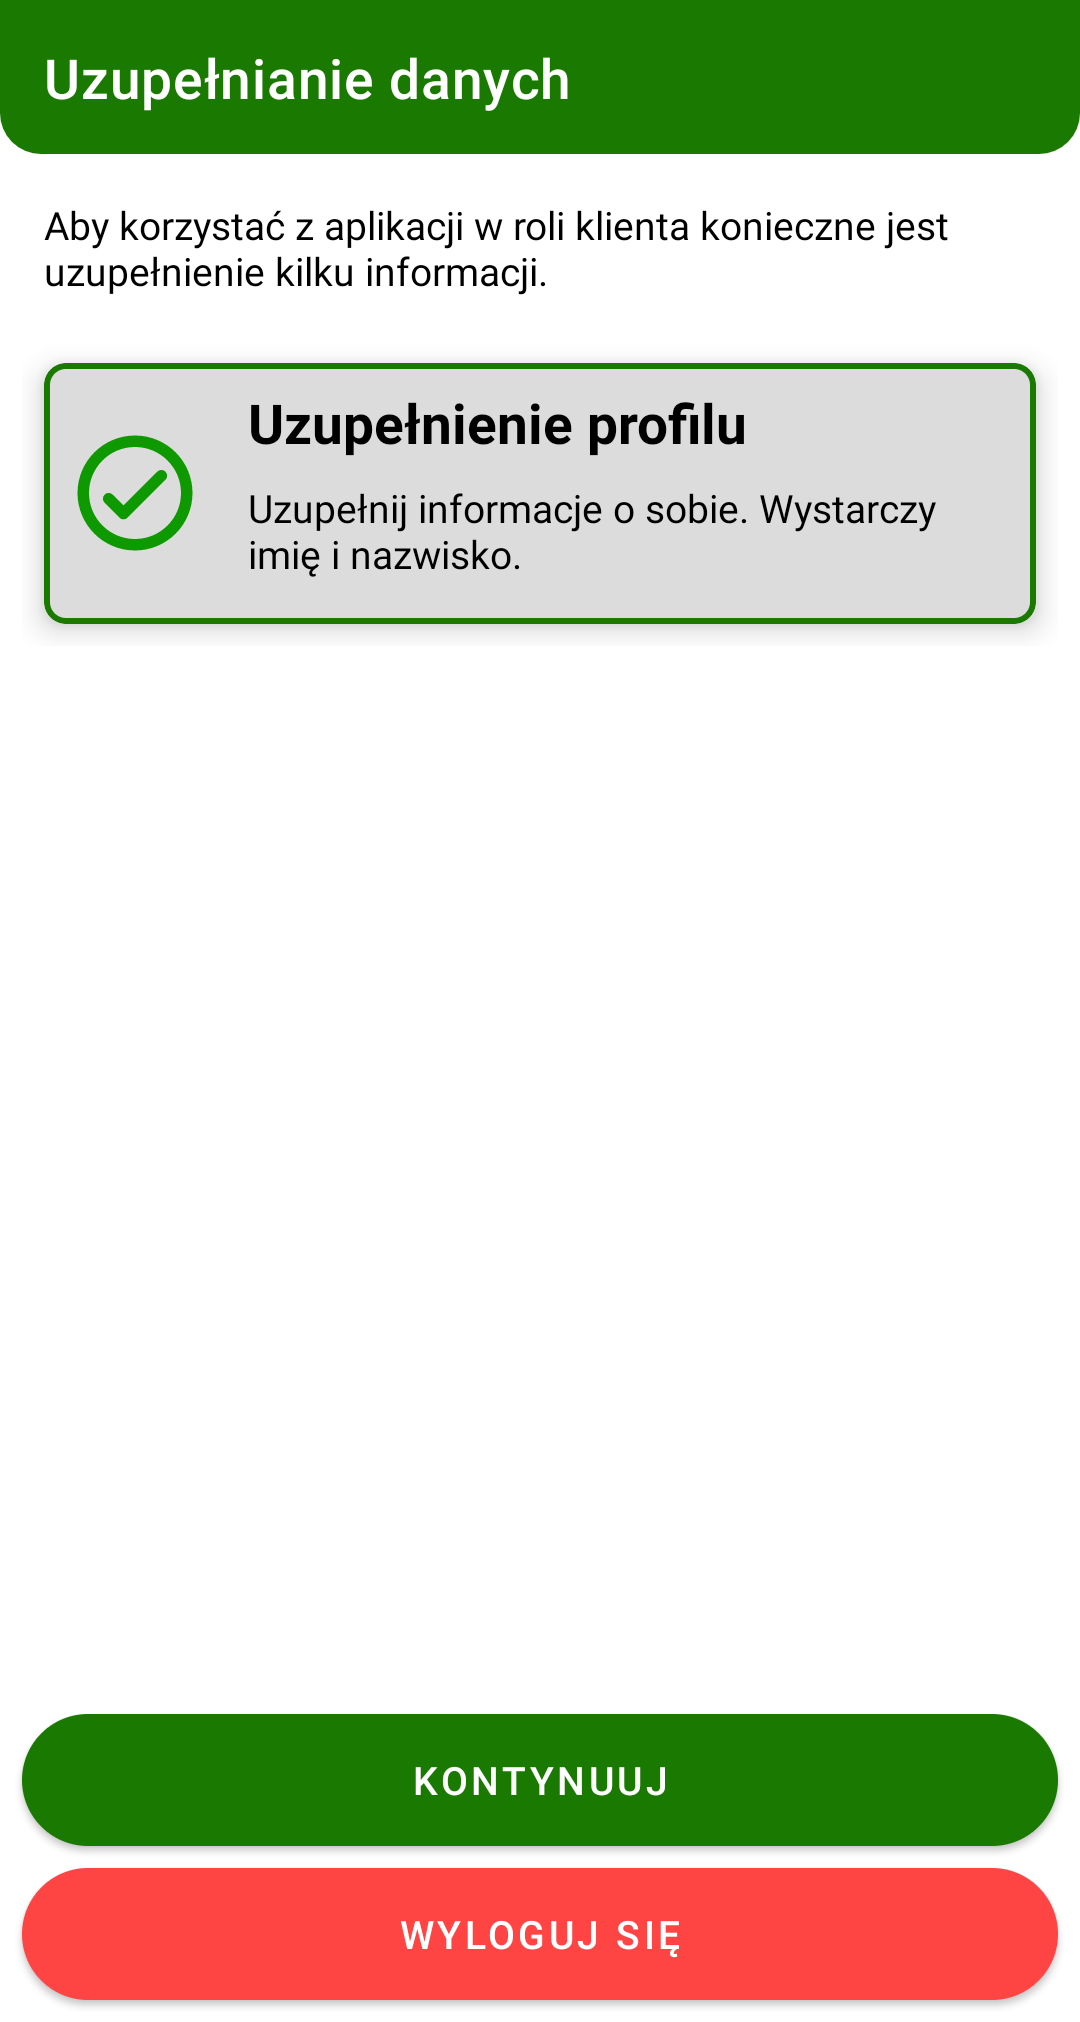
\includegraphics[width=0.97\linewidth]{screens/setup_client.png}}
    \caption{Widok klientów}
  \end{subfigure}
  \begin{subfigure}[t]{0.33\textwidth}
    \centering
    \fbox{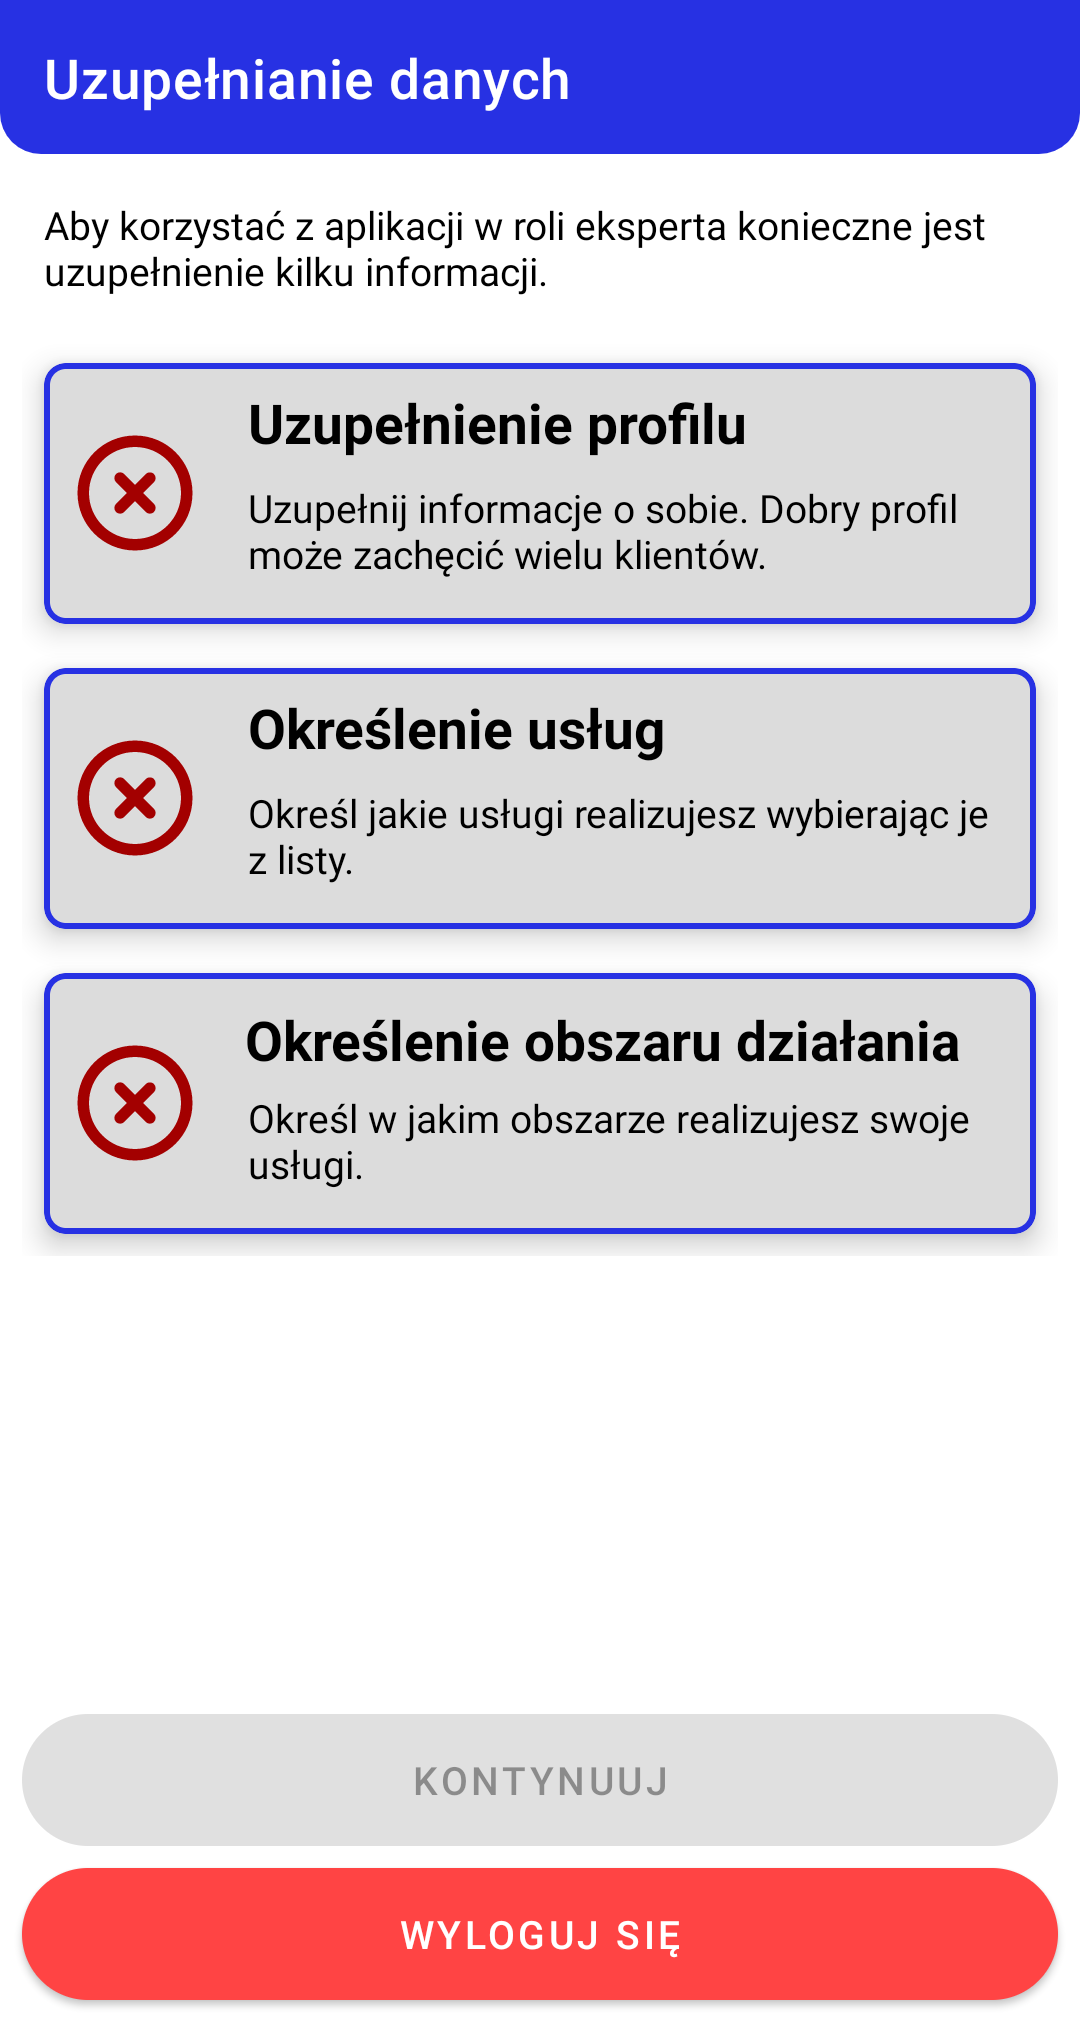
\includegraphics[width=0.97\linewidth]{screens/setup_expert.png}}
    \caption{Widok wykonawców}
  \end{subfigure}
  \caption{Ekrany uzupełniania danych}
  \label{fig:setup}
\end{figure}

Ekrany uzupełniania danych składają się z listy kart, z których każda zawiera informację o akcji koniecznej do podjęcia. Obok nich są również umieszczone ikonki, które mówią, czy zostały już wykonane. Można tego dokonać poprzez wybranie karty, co spowoduje przeniesienie do części aplikacji, która umożliwia modyfikację koniecznych danych. Po ich zatwierdzeniu nastąpi powrót i przy odpowiedniej karcie ikonka krzyżyka zmieni się na ikonkę ptaszka, mówiąc o powodzeniu operacji. Gdy użytkownik spełni wszystkie warunki, to przycisk kontynuacji stanie się aktywny i umożliwi przejście do ekranów głównych. Gdyby jednak nie chciał z jakichś powodów tego zrobić, lecz się wylogować, to również dano mu taką możliwość za pomocą przewidzianego do tego celu przycisku. 